\subsection{Classification Comparison Results}

\subsubsection{Test Set Accuracy}

Table~\ref{tab:classification-comparison} presents the test set performance for all four approaches.
The training-free retrieval baseline is included as an upper reference, though it evaluates on all 13\,325 samples rather than the held-out test set of 2\,000 samples used by the trained classifiers.

\begin{table}[htbp]
\centering
\caption{Classification accuracy on the test set.}
\label{tab:classification-comparison}
\begin{tabular}{lrrrr}
\toprule
\textbf{Approach} & \textbf{Train Samples} & \textbf{Top-1 (\%)} & \textbf{Top-5 (\%)} & \textbf{Top-10 (\%)} \\
\midrule
Retrieval (no training)  & ---     & \textbf{92.17} & \textbf{99.41} & \textbf{99.67} \\
Baseline ResNet-18       & 22\,652 & 83.75          & 96.55          & 97.40          \\
Smart Classical Aug      & 42\,605 & 84.30          & 96.50          & 97.70          \\
Smart Diffusion Aug      & 42\,605 & 79.40          & 94.80          & 96.50          \\
\bottomrule
\end{tabular}
\end{table}

Figure~\ref{fig:test-accuracy-comparison} visualises these results as a grouped bar chart.
Three key findings emerge:

\begin{enumerate}
    \item The training-free retrieval baseline outperforms all trained classifiers, achieving 92.17\% top-1 accuracy without any parameter optimisation.
    \item Smart classical augmentation provides a modest improvement over the ResNet baseline (+0.55\% top-1, +0.30\% top-10), confirming that targeted augmentation of underrepresented classes is beneficial.
    \item Smart diffusion augmentation underperforms the baseline by 4.35\% top-1 and 1.75\% top-5, despite using the same training set size and class-aware targeting.
\end{enumerate}

\begin{figure}[htbp]
    \centering
    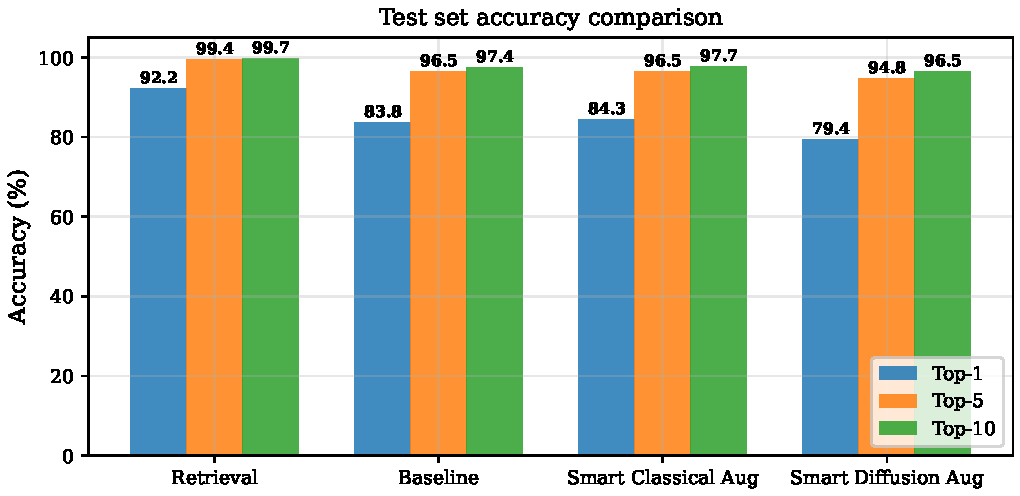
\includegraphics[width=0.95\linewidth]{figures/test_accuracy_comparison.pdf}
    \caption{Grouped bar chart comparing test accuracy across all four approaches: retrieval baseline, ResNet baseline, smart classical augmentation, and smart diffusion augmentation.}
    \label{fig:test-accuracy-comparison}
\end{figure}


\subsubsection{Training Dynamics}

Figure~\ref{fig:training-curves-comparison} overlays the training and validation loss curves for the three trained classifiers.
All models show rapid initial convergence, with training loss stabilising by epoch 80--100.

The diffusion-augmented model exhibits consistently higher validation loss throughout training compared to both the baseline and classical augmentation.
This gap persists from early epochs and does not close with additional training, indicating that the diffusion-generated samples introduce systematic noise rather than useful variation.

The classically augmented model converges within 120 epochs, reaching slightly lower final validation loss than the baseline at 200 epochs.
This is consistent with the augmented data providing genuine additional training signal that helps the model generalise.

\begin{figure}[htbp]
    \centering
    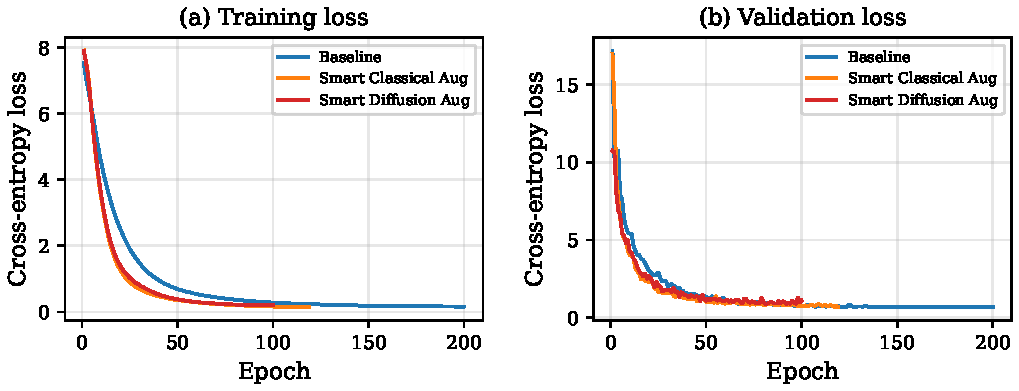
\includegraphics[width=0.95\linewidth]{figures/training_curves_comparison.pdf}
    \caption{Training and validation loss over epochs for the three trained classifiers. The diffusion-augmented model shows persistently higher validation loss.}
    \label{fig:training-curves-comparison}
\end{figure}


\subsubsection{Validation Accuracy Progression}

Figures~\ref{fig:val-top1-comparison}--\ref{fig:val-top10-comparison} show the validation top-$k$ accuracy across training epochs.
The classical augmentation model matches or exceeds the baseline by approximately epoch 60 and maintains a slight advantage thereafter.
The diffusion-augmented model plateaus approximately 5\% below the baseline in top-1 accuracy and does not recover, consistent with the elevated validation loss observed in Figure~\ref{fig:training-curves-comparison}.

The top-5 and top-10 curves show smaller gaps between methods, suggesting that the diffusion augmentation does not fundamentally distort the learned class structure but reduces the model's ability to discriminate among the top candidates.

\begin{figure}[htbp]
    \centering
    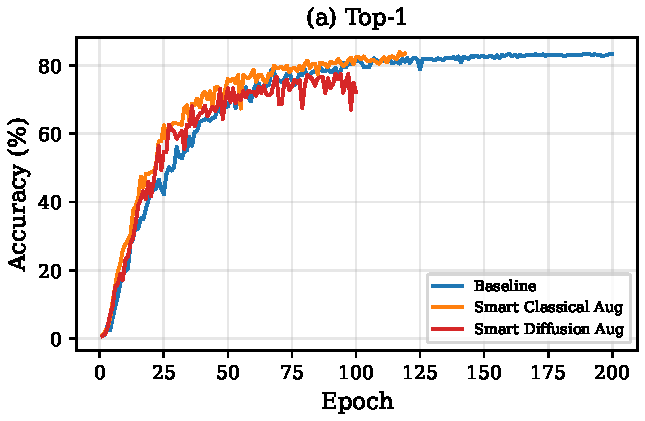
\includegraphics[width=0.85\linewidth]{figures/val_top1_comparison.pdf}
    \caption{Validation top-1 accuracy progression. Classical augmentation matches the baseline by epoch~60, while diffusion augmentation plateaus below.}
    \label{fig:val-top1-comparison}
\end{figure}

\begin{figure}[htbp]
    \centering
    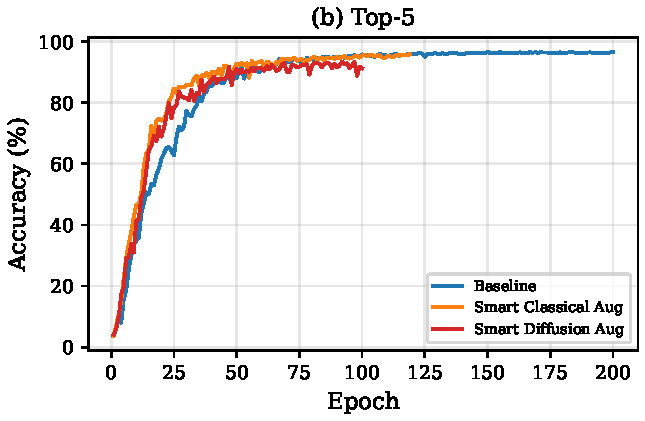
\includegraphics[width=0.85\linewidth]{figures/val_top5_comparison.pdf}
    \caption{Validation top-5 accuracy progression. All three models converge to similar levels, with the diffusion-augmented model trailing slightly.}
    \label{fig:val-top5-comparison}
\end{figure}

\begin{figure}[htbp]
    \centering
    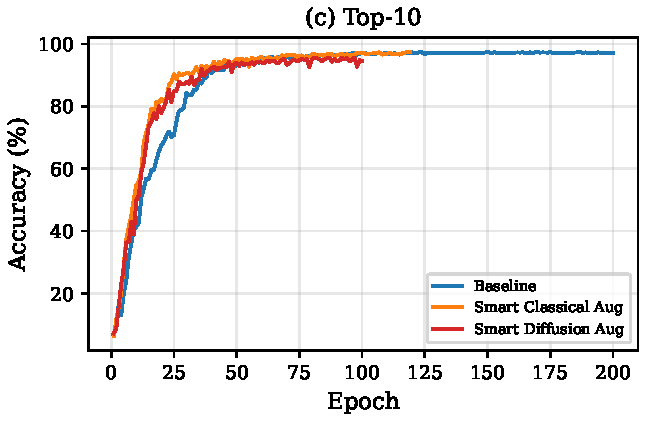
\includegraphics[width=0.85\linewidth]{figures/val_top10_comparison.pdf}
    \caption{Validation top-10 accuracy progression. The gap between methods narrows further at top-10, confirming that diffusion augmentation preserves broad class structure.}
    \label{fig:val-top10-comparison}
\end{figure}
